\documentclass[12pt]{article}
%%% DOCUMENT FORMATTING %%%
\usepackage[margin=1in]{geometry}
\usepackage{enumitem}
\setlength{\parindent}{0pt}
\newcommand{\disp}{\displaystyle}

%%% HEADER %%%
\usepackage{fancyhdr}
\pagestyle{fancy}
\fancyhf{}
\lhead{MATH 1080}
\rhead{Vagnozzi}
\cfoot{\thepage}

%%% MATH NOTATION & SYMBOLS %%%
\usepackage{amssymb}
\usepackage{amsmath}
\newcommand{\R}{\mathbb{R}}
\newcommand{\N}{\mathbb{N}}
\newcommand{\Z}{\mathbb{Z}}
\newcommand{\lp}{\left(}
\newcommand{\rp}{\right)}
\newcommand{\ls}{\left[}
\newcommand{\rs}{\right]}
\newcommand{\lb}{\left\{}
\newcommand{\rb}{\right\}}
\newcommand{\arccot}{\text{arccot}}
\newcommand{\arccsc}{\text{arccsc}}
\newcommand{\arcsec}{\text{arcsec}} 

%%% TABLES %%%
\usepackage{colortbl}

%%% GRAPHS %%%
\usepackage{tikz}
\usepackage{pgfplots}
\pgfplotsset{compat=1.15}
\usepgfplotslibrary{fillbetween}
\usetikzlibrary{angles,quotes}

%%% ENVIRONMENTS %%%
\newcommand{\Example}{\paragraph{\Writinghand \hspace{0.1mm} Example.}}
\newcommand{\ExampleCont}{\paragraph{\Writinghand \hspace{0.1mm} Example (continued).}}
\newcommand{\boxenv}[2]{
	\fbox{
	\begin{minipage}{0.97\textwidth}
	\vspace{2mm}	
	\paragraph{#1} #2
	\vspace{2mm}
	\end{minipage}
	}}

%%% FUN THINGS %%%
\newcommand*\tc[1]{\tikz[baseline=(char.base)]{
            \node[shape=circle,draw,inner sep=2pt] (char) {#1};}}
\usepackage{marvosym}

%%% MISC %%%
\usepackage{hyperref}


\setcounter{page}{1}

\begin{document}
\section*{5.5: The Substitution Method (Review)}

\boxenv{Learning Objectives.}{Upon successful review of Section 5.5, you will be able to\dots
		
	\begin{itemize}[leftmargin=6mm]
		\item Answer conceptual questions involving the Substitution Rule.
		\item Evaluate indefinite integrals using substitution.
		\item Evaluate definite integrals using substitution.
		\item Evaluate integrals with $\sin^2x$ and $\cos^2x$.
		\item Find the area of a region using integration that requires substitution.
	\end{itemize}
	\vspace{-4mm}
}

\vspace{5mm}

\subsection*{A Review of u-Substitution}

Recall from Calculus~I the \textbf{substitution method} for integration, also commonly referred to as \textbf{u-substitution}. Applying the substitution method can be thought of as applying the chain rule for differentiation in reverse.

\paragraph{Strategy for Indefinite Integrals.} Suppose we have an indefinite integral of the form 
$$\disp\int f\big(\textcolor{blue}{g(x)}\big) \textcolor{red}{g'(x)}\,dx.$$
\begin{itemize}
\item[\tc{1}] Set $\textcolor{blue}{u=g(x)}$ so that $\textcolor{red}{du=g'(x)\,dx}$.
\item[\tc{2}] The integral may now be expressed as $\disp\int f(\textcolor{blue}{u})\,\textcolor{red}{du}$.
\item[\tc{3}] If $F$ is an antiderivative for $f$, then $\disp\int f(\textcolor{blue}{u})\,\textcolor{red}{du}=F(\textcolor{blue}{u})+C$.
\item[\tc{4}] We can now substitute $\textcolor{blue}{u=g(x)}$ into $F$ to obtain the final result.

$$\int f\big( \textcolor{blue}{g(x)}\big) \textcolor{red}{g'(x)\,dx}=F\big(\textcolor{blue}{g(x)}\big) + C$$
\end{itemize}

\paragraph{Strategy for Definite Integrals.} For definite integrals, the process of $u$-substitution is nearly the same, but we must modify the limits of integration to correspond with the change of variable.

\vspace{5mm}

In other words, if $\textcolor{blue}{u=g(x)}$ and $\textcolor{red}{du=g'(x)\,dx}$, then

$$\int_a^b f\big( \textcolor{blue}{g(x)}\big) \textcolor{red}{g'(x)}\,dx=\int_{u(a)}^{u(b)} f(\textcolor{blue}{u}\big)\,\textcolor{red}{du}.$$

\newpage

\Example $\disp\int\tan x\,dx$

\vspace{37mm}

\Example $\disp\int\frac{x}{1+x^4}\,dx$

\vspace{37mm}

\Example $\disp\int_0^2\frac{2x}{\left(x^2+1\right)^2}\,dx$

\vspace{57mm}

\begin{minipage}{0.5\linewidth}
\begin{center}
	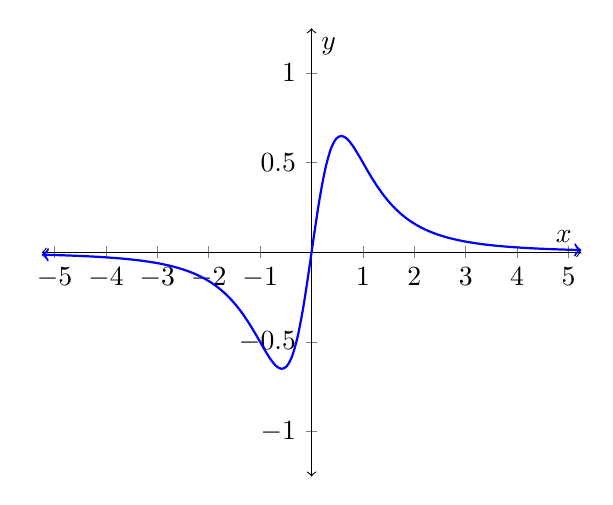
\begin{tikzpicture}
    \begin{axis}[
       	axis x line=center,
       	xmax=5.25, xmin=-5.25,
       	xtick={-5,-4,...,5},
       	axis y line=center,
       	ymax=1.25, ymin=-1.25,
       	ytick={-1,-.5,...,1},
       	xlabel=$x$,ylabel=$y$,
       	axis line style=<->
    ]
    	\addplot[name path=f,smooth,domain=-5.25:5.25,color=blue,samples=100,<->,thick] {(2*x)/(x^2+1)^2};
    \end{axis}
    \end{tikzpicture}
\end{center}
\end{minipage}%
\begin{minipage}{0.5\linewidth}
\begin{center}
	\begin{tikzpicture}
    \begin{axis}[
       	axis x line=center,
       	xmax=5.25, xmin=-5.25,
       	xtick={-5,-4,...,5},
       	axis y line=center,
       	ymax=1.25, ymin=-1.25,
       	ytick={-1,-.5,...,1},
       	xlabel=$u$,ylabel=$y$,
       	axis line style=<->
    ]
    	\addplot[name path=f,smooth,domain=-5.25:-.9,color=blue,samples=100,<->,thick] {1/x^2};
    	\addplot[name path=f,smooth,domain=.9:5.25,color=blue,samples=100,<->,thick] {1/x^2};

    \end{axis}
    \end{tikzpicture}
\end{center}
\end{minipage}

\Example $\disp\int_0^2 x^3\sqrt{16-x^4}\,dx$

\vspace{60mm}

\Example $\disp\int_0^3\frac{w^2+1}{\sqrt{w^3+3w+4}}\,dw$

\vspace{60mm}

\Example $\disp\int_0^{\pi/4}\frac{\sin\theta}{\cos^3\theta}\,d\theta$

\newpage

\Example $\disp\int_0^1 xe^{-x^2}\,dx$

\vspace{60mm}

\Example $\disp\int_0^1\frac{e^z+1}{e^z+z}\,dz$

\vspace{60mm}

\Example $\disp\int_0^4\frac{x}{\sqrt{1+2x}}\,dx$

\end{document}